Below is a plot of $$f(x)=\sin\left(2 \, x + 2\right) + 2 \, \sin\left(-3 \, x\right) - 2 \, \cos\left(-x + 1\right) - 2 \, \cos\left(3 \, x + 2\right) + \cos\left(-x\right) + 1.$$  The {\em \color{red}derivative} of $f(x)$ is the function whose value at $x$ is the {\em slope} of the graph of $f$ at $x$.  Plot the derivative of $f(x)$ by sketching the tangent line to the graph at maybe 10 points, and at each point, plot the slope of that line, then connect your points (it's a good idea to include all points at which the derivative is 0).  There is enough space vertically to fit the derivative.  {\em After} you finish carefully plotting the derivative, enter $f(x)$ into Sage, and plot {\color{blue}\verb|f.derivative()|} to check your work.
\begin{center}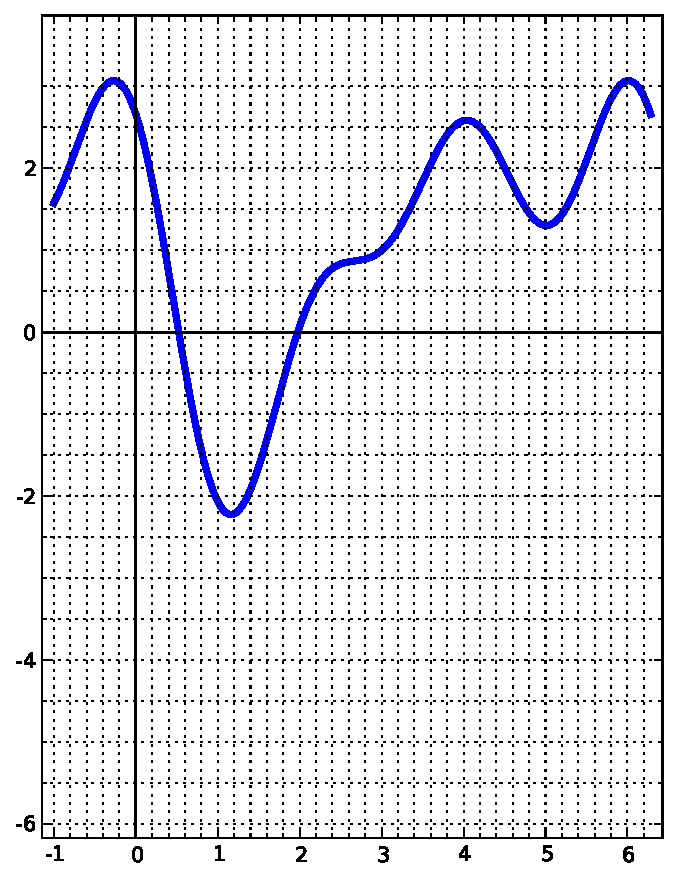
\includegraphics{functions/19.pdf}\end{center}\newpage

